\section{Number theory and cryptography}

\subsection{Divisability}

\begin{definition}
    Divisability: $a|b \iff \thereis k: ak = b$
\end{definition}

\begin{theorem}
    $ a|b \land b|c \then a|c  $
\end{theorem}

\begin{proof}
    \subprf{}{$a|b \land b|c \then a|c$}{
        \subprf{Suppose $ \thereis x_0 : ax_0 = b \land \thereis x_1 : bx_1 = c $}{$\thereis x_2 : ax_2 = c$}{
            Try $ x_2 = x_0 x_1 $ \\
            Then $ a x_2 = a x_0 x_1 = b x_1 = c $
        }
    }
\end{proof}

\begin{theorem}
    If a divides both b and c, then a divides any linear combination of b and c as well.  $ a|b \land a|c \then \forall v, w: a| (vb + wc)  $
\end{theorem}

\begin{proof}
    \subprf{}{$ a|b \land a|c \then \forall v, w: a| (vb + wc)  $}{
        \subprf{Suppose $ a|b \land a|c$}{$\forall v, w: a | (vb + wc)  $}{
            \subprf{Let $v_0, w_0$}{$ \thereis x : ax = (v_0 b + w_0 c) $}{
                Try $ x = v_0 x_0 + w_0 x_1 $
            }
        }
    }
\end{proof}

It is neat how $a|b$ can be read in two ways: 'a divides b', but also 'b is a multiple of a'. This is very nice for interpreting the water-jug problem.
Let $s = \alpha j_1 +\beta j_2$. If there is an $a$ such that $a|j_1 \land a|j_2$ then, by the above proof, $s$ is a multiple of $a$. 

In more common terms, the above condition could be formulated as 'if the basevectors have a common divisor'. As such, the above proof sheds some light on the relation between divisibility and linear combinations. If base-vectors have a common divisor, then they are linearly dependent (proof this for yourself, it's trivial).
The inverse is not always true, however. Consider $2$ and $3$: they have no common divisor (other than 1), yet they are linearly dependent: $\frac{-3}{2}2 + 1 \cdot 3 = 0$

\begin{theorem}
	$ \forall a,b: \thereis ! q, r: a = qb + r \land 0 \leq r \leq q $
\end{theorem}

\begin{theorem}	
    Euclids algorithm: We can simplify the greatest common divisor like this: $ \gcd{a}{b} = \gcd{b}{\rem{a,b}} $
\end{theorem}

\begin{proof}
    \subprf{}{$ \gcd{a}{b} = \gcd{b}{\rem{a,b}} $}{
	    \subprf{}{ $ \CD{a}{b} = \CD{b}{\rem{a}{b}} $ } {
	    	\subprf{ Let $ d_0 \in \CD{a}{b} $ }{ Prove that $ d_0 \in \CD{b}{\rem{a,b}} $ }{
	    	    Since ...	
	    	} 
	    	\subprf{ Let $ d_0 \in \CD{b}{\rem{a}{b}} $ }{ Prove that $ d_0 \in \CD{a}{b} $ }{
	    		Since ...
	    	}
	    }
	    \subprf{}{ Since $ A=B \then \maxOf{A} = \maxOf{B} $, it follows that $ \gcd{a,b} = \gcd{b, \rem{a,b}} $ }{
	    	It is easy to prove that $A \subseteq B \then \maxOf{A} \leq \maxOf{B}$. The reverse holds too, of course. 
	    }
    }
\end{proof}


\begin{proof}
	\subprf{}{$ \forall a,b \thereis \alpha, \beta: \gcd{a}{b} = \alpha a + \beta b $}{
		The proof is not complicated but a little cumbersome. It is given in \href{https://math.stackexchange.com/questions/124891/proof-of-extended-euclidean-algorithm}{this stackexchange post}
	}
\end{proof}

While we have now proven that the gcd can always be expressed as a linear combination of its arguments, we don't know yet just how to obtain the coefficients $\alpha$ and $\beta$. This is where the \emph{extended} euclidian algorithm comes in. 




\subsection{Hashing}

\subsection{Encryption}

\subsubsection{Symmetric encryption}

\subsubsection{Asymmetric encryption}

The basic idea of the Diffie-Hellman algorithm is as follows: instead of a secret key used for encryption and decryption, use a two-part-key. We can then find an algorithm where only the public part of the key is ever visible to Eve. 

Here is an analogy:
\begin{itemize}
	\item You have a lock (pubK) and a key (prvK). Send your lock publically to Bob, while you keep your key hidden in your vest. 
	\item Bob writes his message to you and locks it with your lock in a box. Neither he nor Eve can now open the box again. Bob sends the box to you.
	\item You open the box with your key and read the message
\end{itemize}

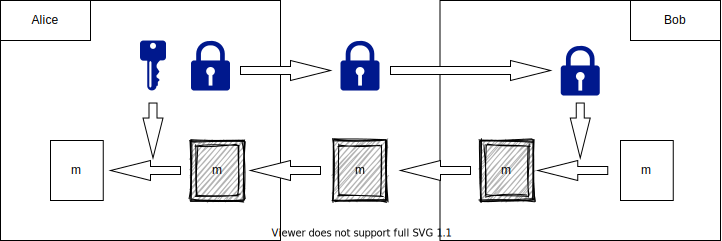
\includegraphics[width=0.6\textwidth]{images/async} 

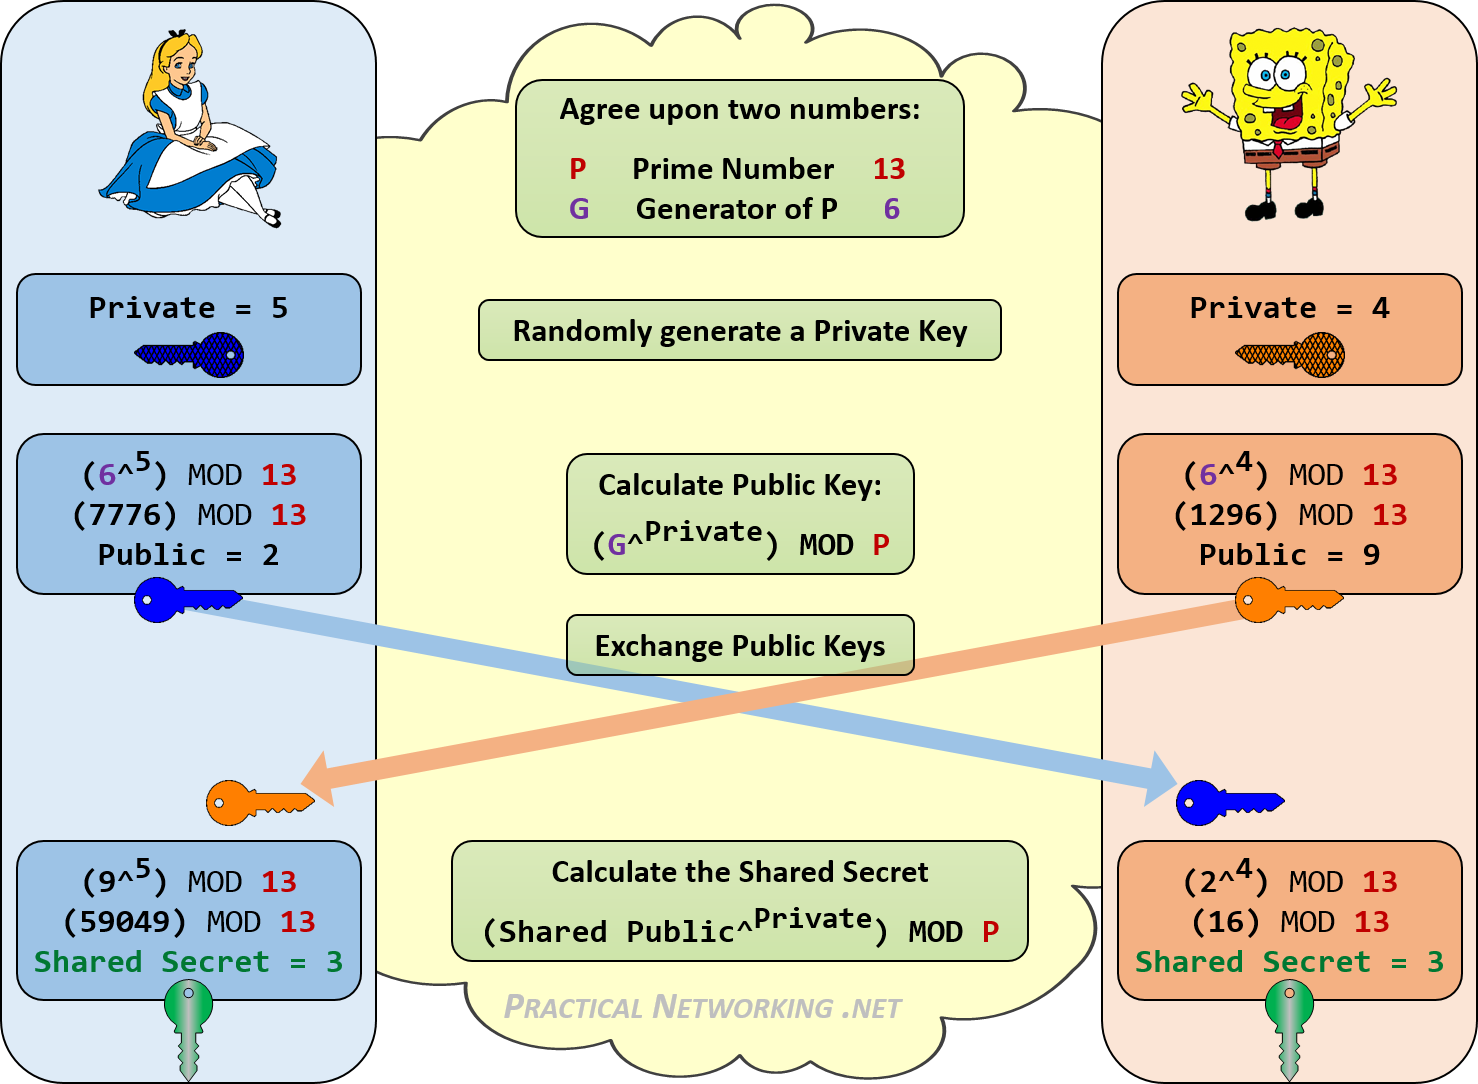
\includegraphics[width=0.6\textwidth]{images/diffie_hellmann} 

This general concept is known as Diffie-Hellman asymmetric encryption. To implement it, one needs 
\begin{itemize}
	\item A function to generate a key-pair
	\item A function for encryption using the message and another persons public key
	\item A function for decryption using a cypher and your own private key
\end{itemize}
The first successful implementation of this principle is known as the WPA algorithm. 

\paragraph{In practice} WPA takes too long to be used very often, whereas symmetric encryption is much faster. For this reason, one usually follows a two step process:
\begin{itemize}
	\item create a new symK
	\item exchange that symK via WPA
	\item use the symK to do symmetric encryption
\end{itemize}

